% !TEX root = ../Dokumentation.tex
\subsection{Fahrbahnerkennung}
\textbf{Funktionsbeschrieb}\\[0.2cm]
Die Fahrbahnerkennung soll primär mittels Kamera umgesetzt werden. Dazu werden Bilder aus dem zur Verfügung gestellten Bilderpool entnommen, mit OpenCV in Graustufen umgewandelt und anschliessend einer Kantenanalyse unterzogen. Dazu wird ein eigener Algorithmus verwendet, der das ganze Bild als Funktion $z = f(x,y)$ anschaut, wobei $x$ der Pixelkoordinate der Spalte, $y$ der Pixelkoordinate der Zeile und $z$ dem Graustufenwert des Pixels entspricht (Abbildung \ref{fig:edges}).
\begin{figure}[H]%Position festigen
\centering
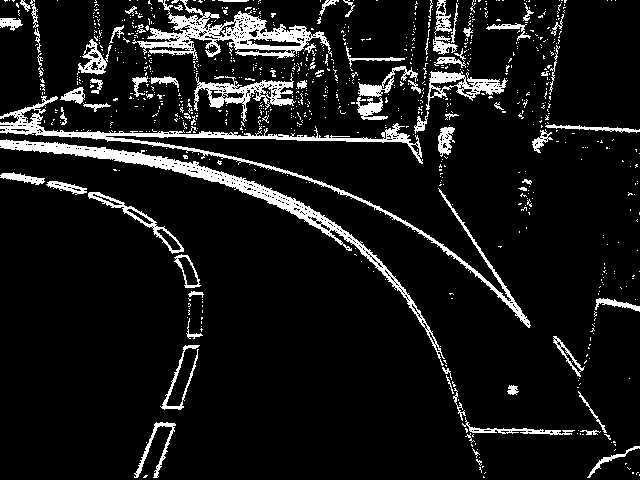
\includegraphics[width=0.6\textwidth]{03_Loesungskonzept/pictures/Kantengrafik.png}
\caption{Bild nach Kantenerkennung}
\label{fig:edges}
\end{figure}
Anhand der vorhandenen Informationen kann die Fahrbahn und demzufolge laufend der Korrekturvektor ermittelt werden. Die eigentliche Korrektur soll mittels PID-Regelung realisiert werden, um eine ruhige Fahrt zu erreichen. Die Korrekturanweisungen werden dabei vom Controller berechnet, und in Grad an das Mikrocontrollerboard weitergegeben.\\[0.2cm]
\newpage
\textbf{Komponentenbeschrieb}
\begin{figure}[H]%Position festigen
\centering
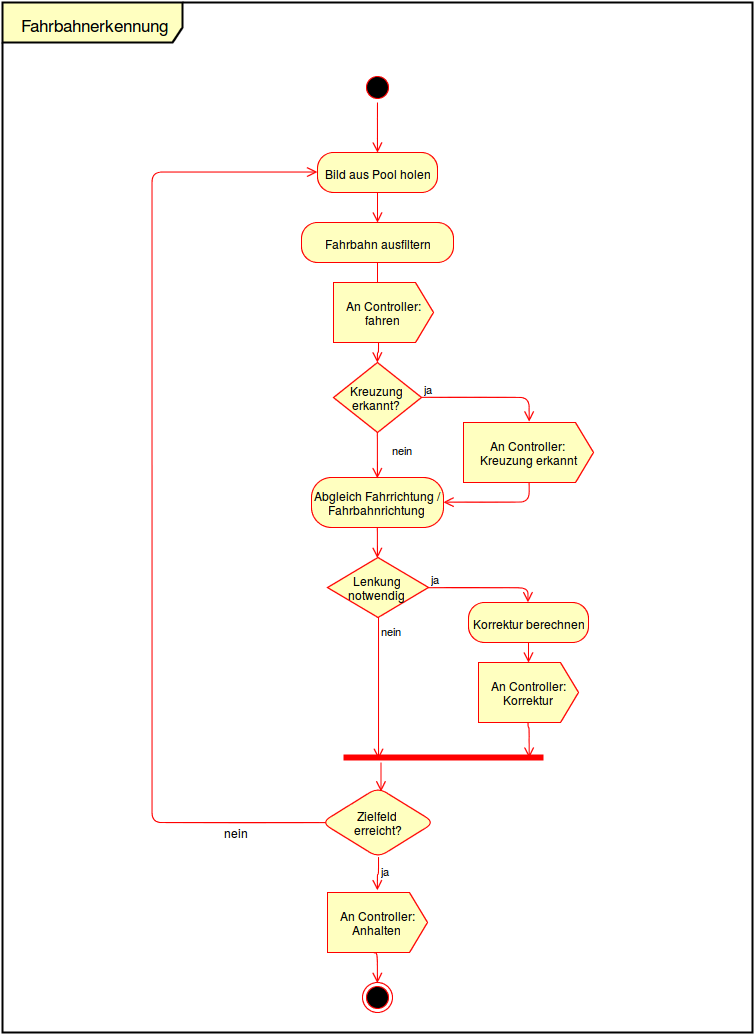
\includegraphics[width=0.7\textwidth]{03_Loesungskonzept/pictures/Fahrbahnerkennung.png}
\caption{Aktivitätendiagramm Fahrbahnerkennung}
\label{fig:activityRoute}
\end{figure}
Die Fahrbahnerkennung wird als eigener Thread auf dem Raspberry Pi realisiert und in C++ objektorientiert umgesetzt. Die erhaltenen Bilder werden vor der Analyse auf ein Format von 320x230 Pixel verkleinert. Für die Kantenerkennung ein Bild zeilenwiese durchlaufen und die Änderungsrate der Graustufe des nächsten Pixels rechts davon ($x$-Richtung) und aus der darüberliegenden Zeile ($y$-Richtung) betrachtet. Überschreitet diese den Filterwert, wird eine Kante erkannt und auch deren Richtung festgehalten (Abbildung: \ref{fig:grayscale}).\\
Im Anschluss wird im unteren Bereich des Bildes von innen nach aussen die Fahrbahn gesucht. Dazu werden jeweils von der Bildmitte aus, in beide Richtungen, die ersten Kanten gesucht, über mehrere Punkte fixiert und danach alle übrigen Kanten entfernt.
\begin{figure}[H]%Position festigen
\centering
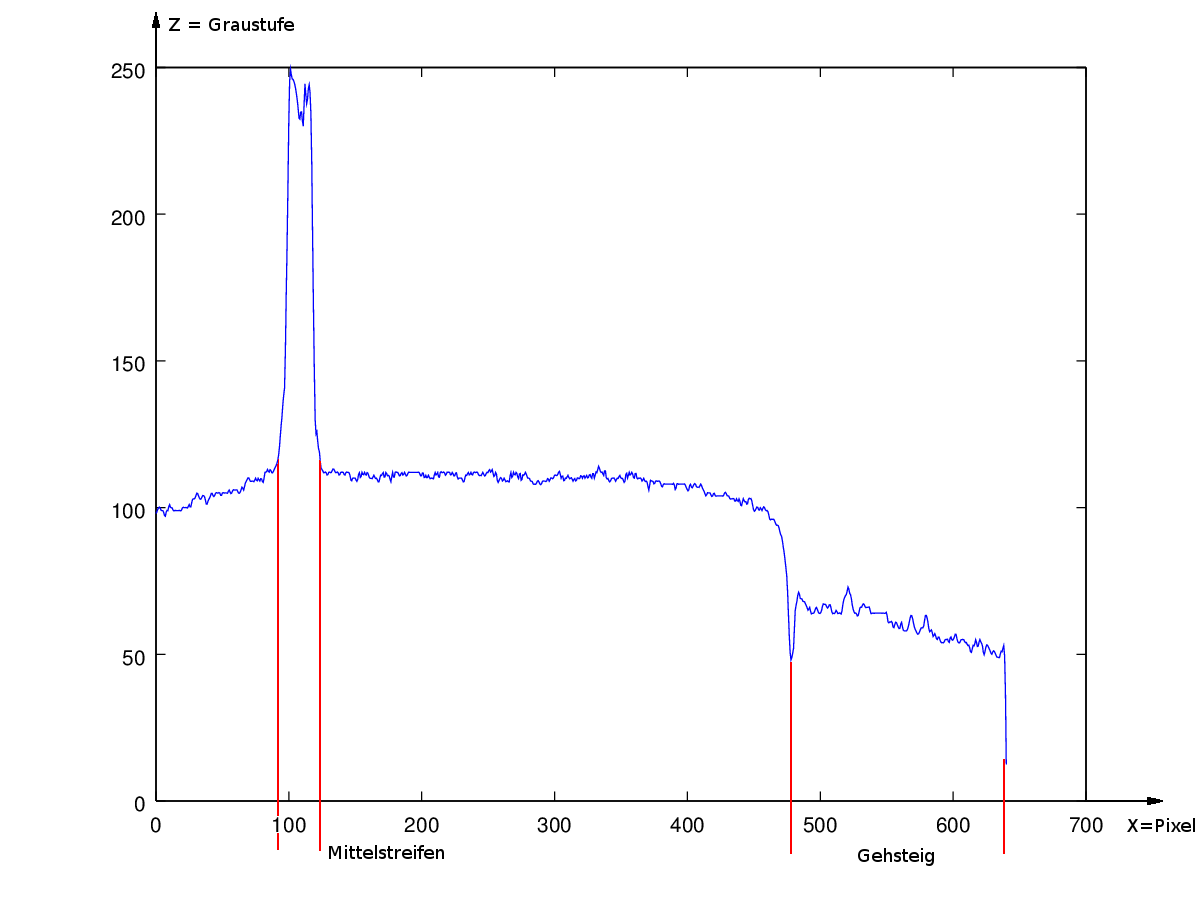
\includegraphics[width=0.6\textwidth]{03_Loesungskonzept/pictures/graphPicture.png}
\caption{Graph der Graustufenwerte einer Bildzeile in $x$-Richtung}
\label{fig:grayscale}
\end{figure}
Da die Fahrbahn keine sprunghaften Änderungen aufweisen kann, wird die kantendetektierte Matrix von unten nach oben durchgesehen und alle Kanten, die in $x$ - Richtung eine zu grosse Abweichung von der erkannten Fahrbahn aufweisen entfernt, so dass nur noch die rechte und linke Fahrbahnbegrenzung übrig bleibt (Abbildung \ref{fig:kantenl} und \ref{fig:kantenr}). Lücken werden geschlossen, indem in Richtung des letzten Elementes fortgefahren wird.\\
Für die anschliessende Suche der Ideallinie wird von den gefundenen Kanten die Mitte genommen. Die Abweichung wird ermittelt, indem der Fahrtrichtungsvektor mit dem Richtungsvektor der Ideallinie abgeglichen wird. Bei einem zu grossen Winkelfehler wird eine Korrektur eingeleitet. In der Kurve wird dazu der Fahrtrichtungsvektor durch einen Bogen, entsprechend dem eingeschlagenen Radius der Lenkung, ersetzt und mit dem Sollradius der Fahrbahn abgeglichen. Die Abweichung wird dann über die Tangentenfunktion in einen Winkel umgewandelt, um für die Regelung nur einen Wertetyp auswerten zu müssen. Da die Kurven, insbesondere auf der Innenbahn, sehr eng sind, verliert die Kamera die Fahrbahn aus der Sicht. Um dieses Problem zu lösen wird die Kamera beim Kurveneingang auf einen festgelegten und konstanten Winkel gedreht, der dann wiederum in der Regelung beachtet werden muss. Am Ende der Kurvenfahrt wird die Kamera wieder auf die Null-Grad-Position zurückgeschwenkt. Nebst der besseren Fahrbahnsicht werden auch Objekte auf diese Weise früher erkannt.
\begin{figure}[H]
\centering
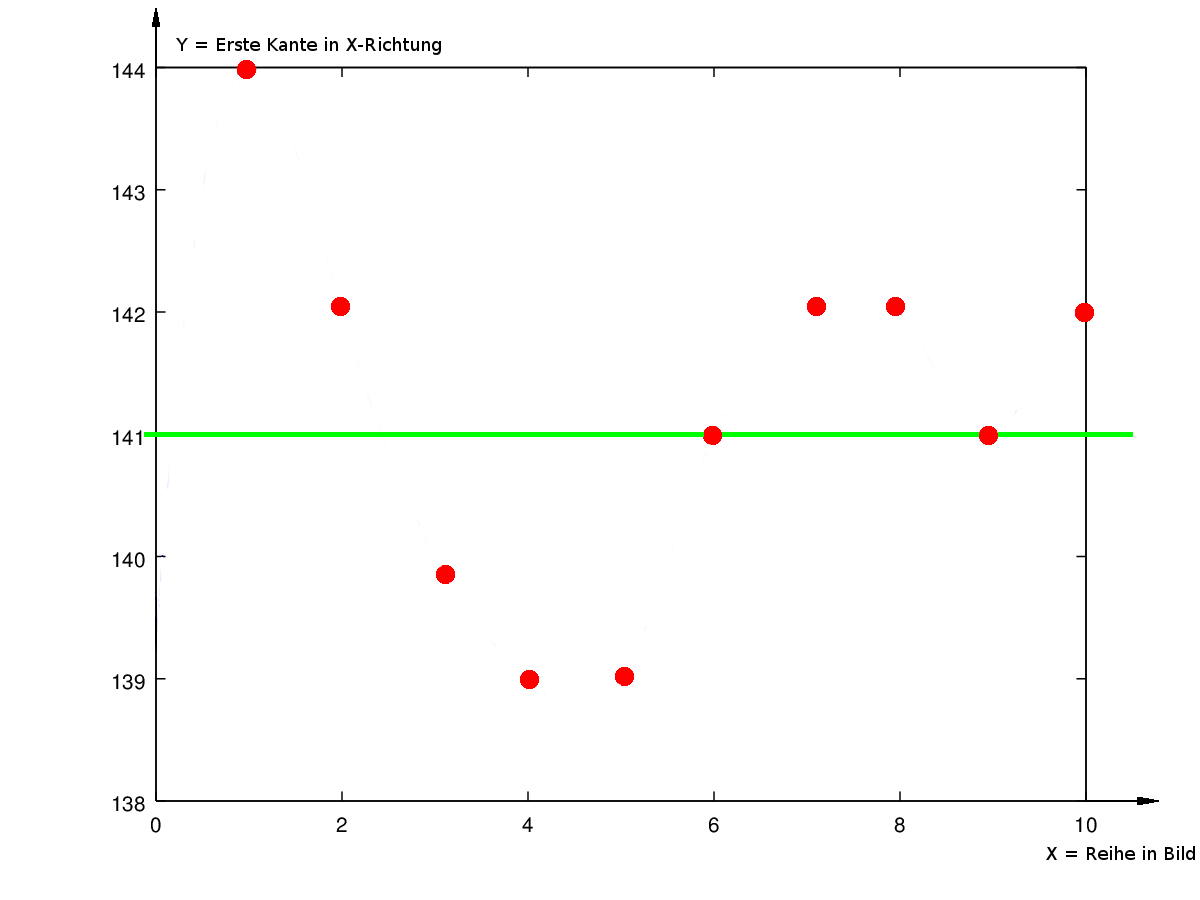
\includegraphics[width=0.6\textwidth]{03_Loesungskonzept/pictures/minEdge.png}
\caption{Erste Kante links der Mitte}
\label{fig:kantenl}
\end{figure}
\begin{figure}[H]
\centering
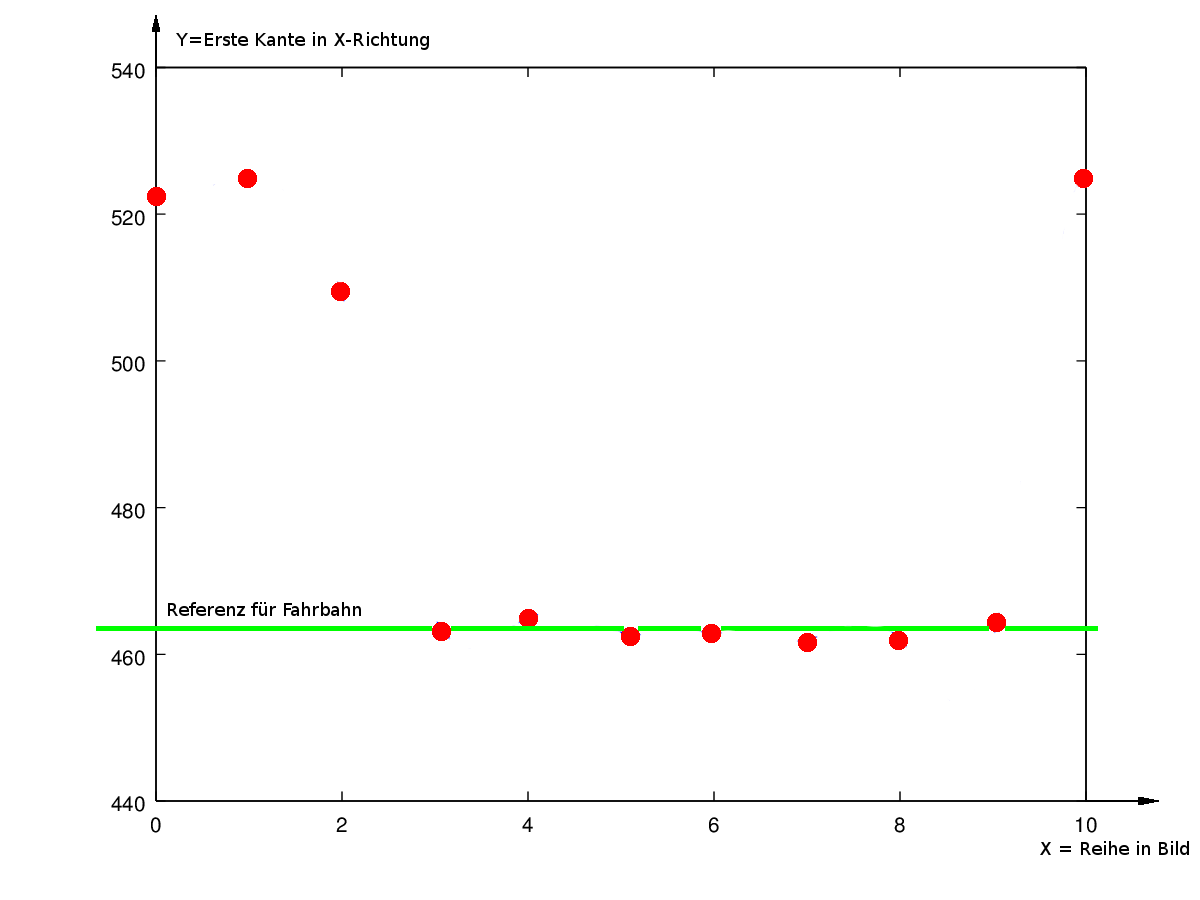
\includegraphics[width=0.6\textwidth]{03_Loesungskonzept/pictures/maxEdge.png}
\caption{Erste Kante rechts der Mitte}
\label{fig:kantenr}
\end{figure}
\textbf{Begründung}\\[0.2cm]
Mit der beschriebenen Vorgehensweise kann der Aufwand pro Bild gegenüber OpenCV deutlich reduziert werden, da die Operationen ausschliesslich für die Fahrbahnerkennung erstellt werden. Die Tests haben die Realisierbarkeit dieser Vorgehensweise als machbar und fexibel aufgezeigt.\\[0.2cm]
\textbf{Berechnungen}\\[0.2cm]
Abschätzung der Komplexität des Algorithmus: Jedes Bild wird als eine $n\times{m}$ Matrix $M$ betrachtet, wobei $n$ = Spaltenzahl und $m$ = Zeilenzahl. Die Resultate der Kantenerkennung werden in einer zweiten $n\times{m}$ Matrix $M_1$ gespeichert, welche für die weiteren Berechnungen verwendet wird. Anhand des Bildformates gilt: $n>m$. Die Umwandlung des Bildes in Graustufen, von OpenCV durchgeführt, ist in der Abschätzung nicht enthalten.
\begin{itemize}
\item Iteration für Kantenerkennung:
\[
n \cdot m \leq n \cdot n \text{ wenn } n\geq m \rightarrow \mathcal{O}(n^2) \text{ mit den Zeugen }C=1 \text{ und } k = 1
\]
\item Iteration für Kantenfindung Fahrbahn:
\[
\frac{1}{2}(10n) + \frac{1}{2}(10n) = 5n + 5n = 10n \rightarrow \mathcal{O}(n) \text{ mit den Zeugen }C=10 \text{ und } k = 1
\]
\item Iteration für Fahrbahnausfilterung und das Erzeugen der Sollspur:
\[
n \cdot m \leq n \cdot n \text{ wenn } n\geq m \rightarrow \mathcal{O}(n^2) \text{ mit den Zeugen }C=1 \text{ und } k = m
\]
\item Zusammengezogene Schätzung der Komplexität:
\begin{align*}
2(n^2) + 10n &\leq 2n^2 + 10n^2 \text{ wenn } n\geq 1\\
             &= 12n^2\\
             &\rightarrow \mathcal{O}(n^2) \text{ mit den Zeugen }C=12 \text{ und } k = m
\end{align*}
\end{itemize}
Formeln für die Berechnungen:
\begin{itemize}
\item Kantenfindung $h=$ Grenzwert für die Änderungsrate um eine Kante zu ermitteln und $z_1$ der Wert des Pixels in der Quellmatrix $M$:
$z = f(x,y) = \text{ Graustufen des Pixels }0 \leq z \leq 255$\\
\[
\frac{\partial{z}}{\partial{x}}=\frac{f(x+\Delta{x})-f(x)}{\Delta{x}} = \frac{f(x+1)-f(x)}{1} = f(x+1)-f(x)
\]
\[
\frac{\partial{z}}{\partial{y}}=\frac{f(y+\Delta{x})-f(y)}{\Delta{y}} = \frac{f(y+1)-f(y)}{1} = f(y+1)-f(y)
\]
\[
\nabla f(x,y) = \begin{bmatrix}
\frac{\partial{z}}{\partial{x}}\\
\frac{\partial{z}}{\partial{y}}
\end{bmatrix}
\]
\[
\lVert\nabla f(x,y)\rVert = \sqrt{(f(x+1)-f(x))^2 + (f(y+1) - f(y))^2}
\]
Wenn nun der $\lVert\nabla f(x,y)\rVert \geq h$ , wird in die Zielmatrix $M_1$ an die Stelle $(x,y)$ der Wert 255 geschrieben, sonst 0.
\item Finden der Fahrbahnreferenz am unteren Bildrand:\\
Wie zuvor beschrieben wird für die Fahrbahn von innen nach aussen gesucht. Dabei wird jeweils die erste Kante genommen, für die gilt:
\[
\frac{\partial{z}}{\partial{y}} > h_y
\]
wobei $h_y$ für die minimale erwartete Änderung in $y$-Richtung steht. Im Anschluss werden die $min_x$- und $max_y$-Koordinaten der gefundenen Limits folgendermassen angeglichen:
\[
min_{(x,y)} = 10\cdot\Bigl\lfloor\frac{min_{(x,y)}}{10}+0.5\Bigr\rfloor
\]
respektive:
\[
max_{(x,y)} = 10\cdot\Bigl\lfloor\frac{max_{(x,y)}}{10}+0.5\Bigr\rfloor
\]
\end{itemize}
Die Fahrbahnkanten werden im Anschluss anhand der ermittelten Werte gesucht. Ist eine Kante in der Nähe der ermittelten Fahrbahn, wird sie behalten, ansonsten entfernt. Der Grenzwert muss noch genau ermittelt werden.\\
Die Parameter für die Regelung werden mit folgender Formel ermittelt:
\[
G_R = K_p\left(1 + \frac{1}{T_{n^S} + T_{v^S}}\right)
\]
Danach werden die ermittelten Werte in die Korrekturformel eingesetzt:
\[
y = K_{PR}\left(e + \frac{1}{T_n}\int{edt} + T_v\dot{e}\right)
\]
wobei $y$ dem zu korrigierenden Winkelwert in Grad entspricht. Die Parameter $T_v$, $T_n$ und $K_{PR}$ müssen für die Feineinstellung justierbar sein. Dies soll für die Debugphase über eine auf dem Notebook betriebene Software geschehen.
\\[0.2cm]
\textbf{Testergebnisse}\\[0.2cm]
In den bisher durchgeführten Tests konnten die Bilder der Kamera mit einer Framerate von 10 - 20 Bilder auf dem Minicomputer verarbeitet werden. Die Lichteinflüsse haben sich dabei als handhabbar präsentiert, wenn die Beleuchtung mindestens der im Testgebäude vorhandenen Standardbeleuchtung entspricht. Hellere Lichtverhältnisse haben sich positiv auf die Kantenerkennung ausgewirkt.\\
Die Parallelisierung hat sich ebenfalls erfolgreich testen lassen, gemeinsam mit der Objekterkennung, allerdings nur auf dem Notebook aufgrund einer defekten Testkamera.
\\[0.2cm]
\newpage
\underline{\textbf{Fahrbahnerkennung Unterstützung}}
\\[0.2cm]
\textbf{Funktionsbeschrieb}\\[0.2cm]
Wird die Fahrbahn auf einer Seite ganz verloren, speziell in engen Kurven, dann wird die Erkennung an den Flexsensor übergeben, der mit dem seitlichen Abstand zum Trottoir die Fahrspur halten soll.\\[0.2cm]
\textbf{Komponentenbeschrieb}\\[0.2cm]
\begin{figure}[H]
	\centering
	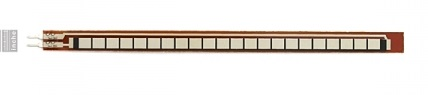
\includegraphics[width=0.5\textwidth]{03_Loesungskonzept/pictures/Flexsensor.jpg}
	\label{fig:Flexsensor}
	\caption{Flexsensor}
\end{figure}%
Der Flexsensor ändert seinen Widerstandswert abhängig davon, wie stark der Sensor gebogen wird. \\[0.2cm]
%
\textbf{Begründung}\\[0.2cm]
Für die Distanzmessung zum Trottoir wurden noch andere Sensoren (Ultraschall und Infrarot-Sensor) in Betracht gezogen. Jedoch sind die Ultraschall-Sensoren zu unpräzise und die Infrarot-Sensoren haben Mühe mit der schwarzen Oberfläche des Trottoirs. Beides wurde mit einem Funktionsmuster ausgetestet. Der Flexsensor hat bei beiden diesen Punkten bessere Eigenschaften.\\[0.2cm]
\textbf{Testergebnisse}\\[0.2cm]
Diese Kennlinie stellt den Widerstandswert in Funktion von dem Biegewinkel dar.
\begin{figure}[H]
	\centering
	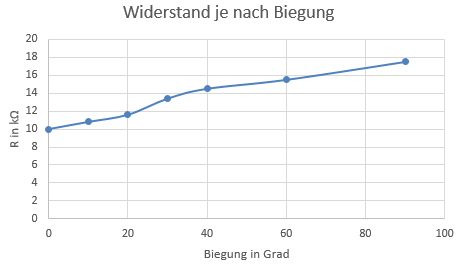
\includegraphics[width=0.5\textwidth]{03_Loesungskonzept/pictures/Flex_Biegungskennline.png}
	\label{fig:Flex_R_Kennlinie}
	\caption{Widerstand in Funktion des Biegewinkels}
\end{figure}
%
Mit dieser Widerstandsänderung kann auf die Distanz geschlossen werden. Die Berechnung oder Auswertung welcher Widerstandswert zu welcher Distanz passt muss noch im PREN2 gemacht werden. Der Widerstandswert des Flexsensors kann über einen einfachen Spannungsteiler und einem AD-Wandler eingelesen werden.
Ein Risiko besteht darin, dass der Flexsensor auf das Trottoir springt, anstatt sich zu biegen. Jedoch sollte dies durch eine optimale Positionierung vermieden werden können.